%Authors guidlines: http://royalsocietypublishing.org/instructions-authors
% 2500 words max (includes the title page, abstract, references, acknowledgements and figure/table legends)
% current version is around 3700. I think a big cut down can be done on the references.
% We allow a maximum of 4 displays, only 2 of which can be figures.

\documentclass[12pt,letterpaper]{article}


%Packages
\usepackage{pdflscape}
\usepackage{fixltx2e}
\usepackage{textcomp}
\usepackage{fullpage}
\usepackage{float}
\usepackage{latexsym}
\usepackage{url}
\usepackage{epsfig}
\usepackage{graphicx}
\usepackage{amssymb}
\usepackage{amsmath}
\usepackage{bm}
\usepackage{array}
%\usepackage{mhchem}
\usepackage{ifthen}
\usepackage{caption}
\usepackage{hyperref}
\usepackage{amsthm}
\usepackage{amstext}
\usepackage{enumerate}
\usepackage[osf]{mathpazo}
\usepackage{dcolumn}
\usepackage{lineno}
\usepackage{longtable}

\pagenumbering{arabic}

\newcolumntype{L}[1]{>{\raggedright\let\newline\\\arraybackslash\hspace{0pt}}m{#1}}
\newcolumntype{C}[1]{>{\centering\let\newline\\\arraybackslash\hspace{0pt}}m{#1}}
\newcolumntype{R}[1]{>{\raggedleft\let\newline\\\arraybackslash\hspace{0pt}}m{#1}}

%Pagination style and stuff % NC: Note that these are all syst biol specific.
\linespread{2}
\raggedright
\setlength{\parindent}{0.5in}
\setcounter{secnumdepth}{0} 
\renewcommand{\section}[1]{%
\bigskip
\begin{center}
\begin{Large}
\normalfont\scshape #1
\medskip
\end{Large}
\end{center}}
\renewcommand{\subsection}[1]{%
\bigskip
\begin{center}
\begin{large}
\normalfont\itshape #1
\end{large}
\end{center}}
\renewcommand{\subsubsection}[1]{%
\vspace{2ex}
\noindent
\textit{#1.}---}
\renewcommand{\tableofcontents}{}
%\bibpunct{(}{)}{;}{a}{}{,}

%---------------------------------------------
%
%       START
%
%---------------------------------------------

\begin{document}

%Running head
\begin{flushright}
Version dated: \today
\end{flushright}

\bigskip
\medskip
\begin{center}

\noindent{\Large \bf Do Natural History Docuementaries Prompt Public Engagement?} 

\bigskip

\noindent {\normalsize \sc Adam Kane$^1$ and Dario Fernandez-Bellon$^1$}\\
\noindent {\small \it 
$^1$Biological, Earth and Environmental Sciences, University College Cork, Cork, Ireland}\\

\end{center}
\medskip
\noindent{*\bf Corresponding author.} \textit{adam.kane@ucc.ie}\\  
\vspace{1in}

%Line numbering
\modulolinenumbers[1]
\linenumbers

%---------------------------------------------
%
%       ABSTRACT
%
%---------------------------------------------
\begin{abstract}
\end{abstract}

\noindent Key words: conservation, documentaries, public engagement\\


%---------------------------------------------
%
%       INTRODUCTION
%
%---------------------------------------------

\newpage 
\section{Introduction}
We live in the Anthropocene, one of the most critical times for our species and the planet. But we also live in a time of constant technological change, instant rewards and short attention spans. Conservation biologyis faced with broaching this issue, and making acquiredknowledgeon the state of biodiversity and solutions to avoid or minimise the 6th extinction accessible to the general public. Documentaries have recently shown their potential to fill this role, with viewing figures at record levels.But we wonder whether they are actually getting the message across, or if it is lost along the way, and if so, where that loss is/ how we can improve the quality and reach of the message.

"As a conservationist, I think I would be doing the cause a great disservice if I tacked on to the end of every single programme that I did, a little homily to explain yet again that mankind is wrecking the environment that I have been showing. My job as a natural history film make is to convey the reality of the environment so that people will recognise its value, its interest, its intrinsic merit and feel some responsibility for it. After that has been done, then the various pressure groups can get at them through their own channels and ask them to send a donation to, let us say, the World Wildlife Fund." \cite{burgess1984exploring}.

"There are two planet earths. One of them is the complex, morally challenging world in which we live, threatened by ecological collapse. The other is the one we see on the wildlife programmes." George Monbiot

"The loss of wilderness is a truth so sad, so overwhelming that, to reflect reality, it would need to be the subject of every wildlife film. That, of course, would be neither entertaining nor ultimately dramatic. So it seems that as filmmakers we are doomed either to fail our audience or fail our cause."
Stephen Mills (1997)

%---------------------------------------------
%
%       METHODS
%
%---------------------------------------------
\section{Materials and Methods}
Firstwe lookat the potential of docs to impact / generate public awarenessa.Sequence time (or no words) and number of original tweets and wiki hits. Then we look at whether docs are actually reflecting what occurs in the natural world, or as recent criticism suggests, represents a fictitious picture of the state of the plane. a.IUCN vertebrate status -> reflected in script? -> reflected in twitter volume or sentiment?-> reflected in wiki hits? b.Total time / words dedicated to cons messages (including overview sequences) c.Figure with map of distribution of stories, taxa breakdown and IUCN status breakdown. Finally, we look at whether this awareness actually results in engagement and has an impact on conservation issues. Case studies of specific sequences and web hits/donations to relevant charities

%---------------------------------------------
%
%       RESULTS
%
%---------------------------------------------


\section{Results}

\begin{figure}[H]
\centering
    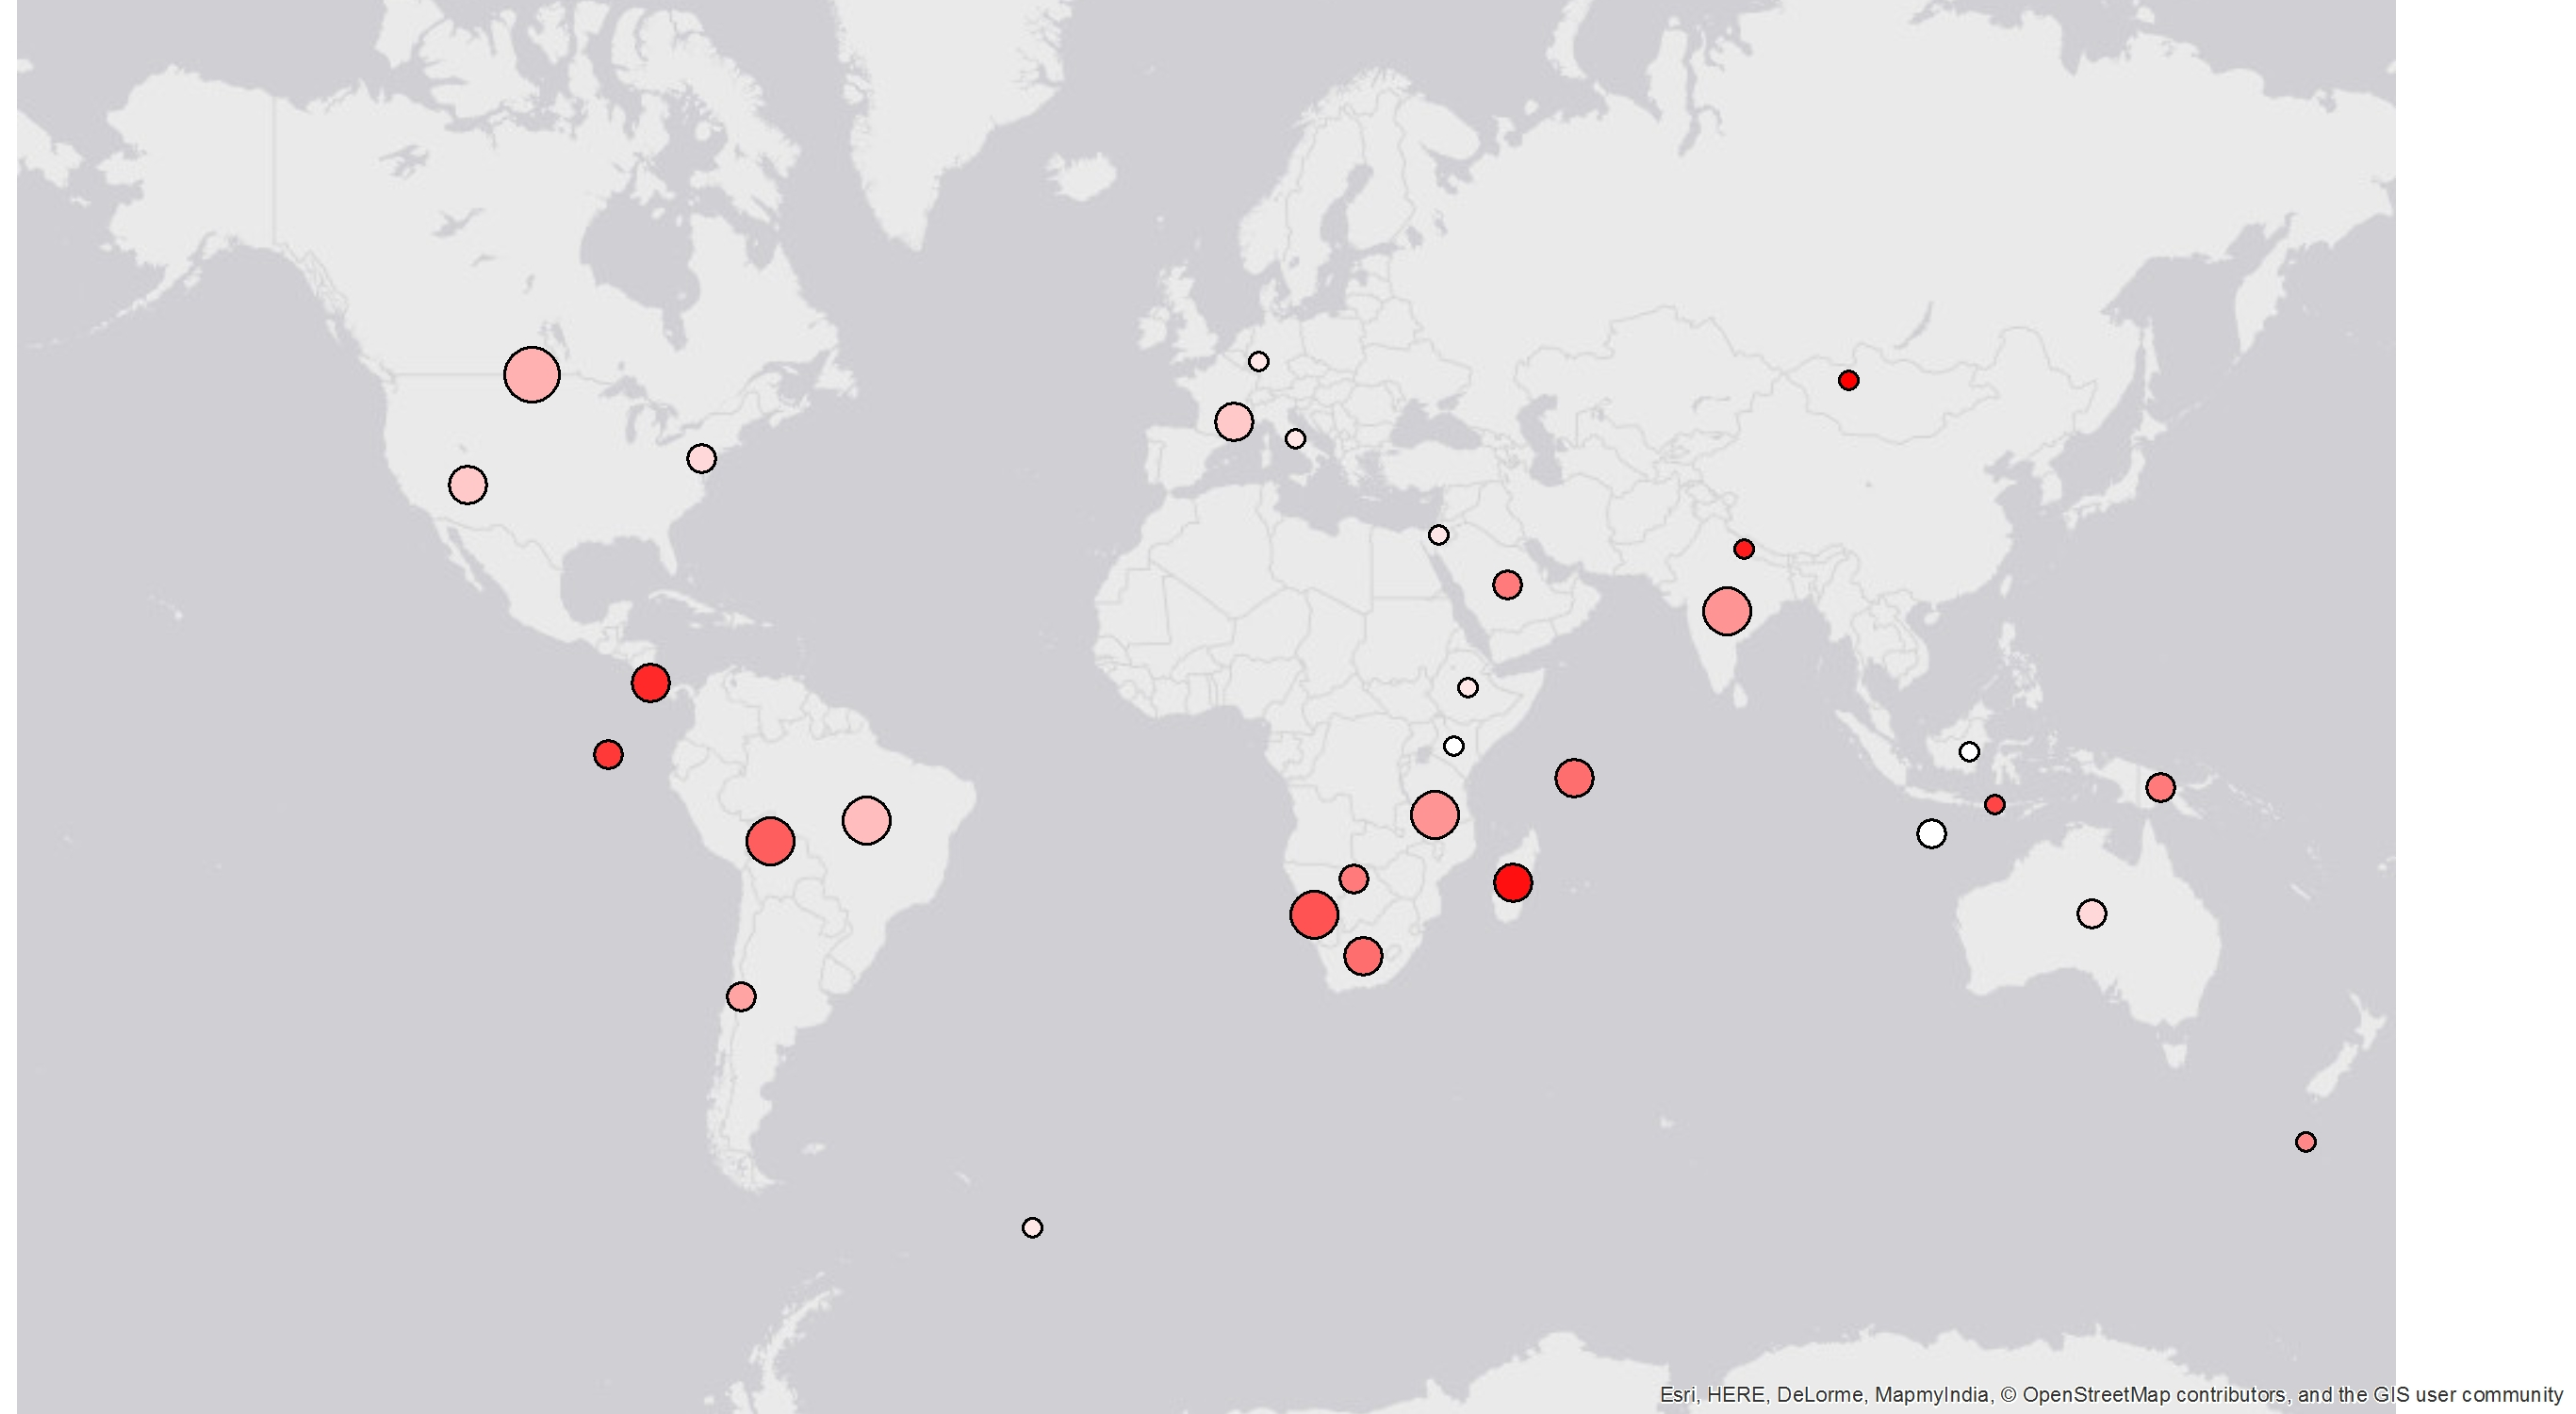
\includegraphics[keepaspectratio, totalheight=0.5 \textheight]{map2.jpg}
\caption{Average IUCN status of species featured on Planet Earth 2}
\label{info.diff}
\end{figure}


%---------------------------------------------
%
%       DISCUSSION
%
%---------------------------------------------

\section{Discussion}

%Biology letters various stuff
\section{Ethics statement}
N/A
\section{Data accessibility statement}
All data and analysis code is available on GitHub (\url{https://github.com/kanead}).
\section{Authors' Contributions}
All authors approved the final version of the manuscript.
\section{Competing Interests}
We have no competing interests.
\section{Acknowledgments}
We thank Sir David and Amy Cooke for emotional support.

\bibliographystyle{vancouver}
\bibliography{References}

%END
\end{document}
